\subsection{Designing the Controller Under Constraint}
In this part, we aim to find a PD controller that conforms with the design requirements needed. In order to achieve such a configuration, we used the Root Locus method and chose our $K_p$ and $K_d$ values accordingly. Figure \ref{fig:dr1} below shows the root locus with the vertical line showing the $T_s < 4$ threshold. I should be kept in mind that due to location of zero, we might not satisfy the condition even if all our poles are in the safe region. Therefore, we checked the settling time from the step response to be safe. 

\begin{figure}[H]
    \centering
    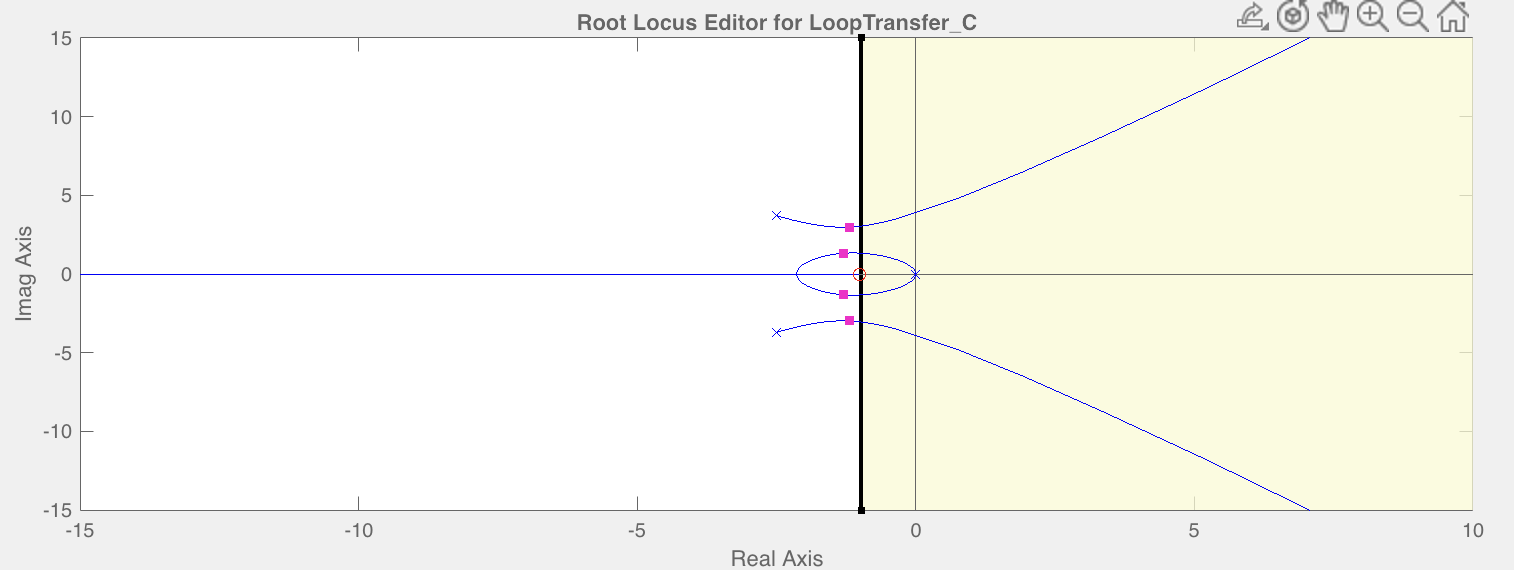
\includegraphics[width=.8\textwidth]{images/dr_1.png}
    \caption{$T_s < 4$ seconds}
    \label{fig:dr1}
\end{figure}

Following this, we added an extra constraint on the percent overshoot metric. Since percent overshoot is a function of damping ratio, this constraint is not a vertical line, but 2 lines originating from zero in negative real axis quadrants. The snapshot of CSD showing the constraints together are shown on Figure \ref{fig:dr2}. 

\begin{figure}[H]
    \centering
    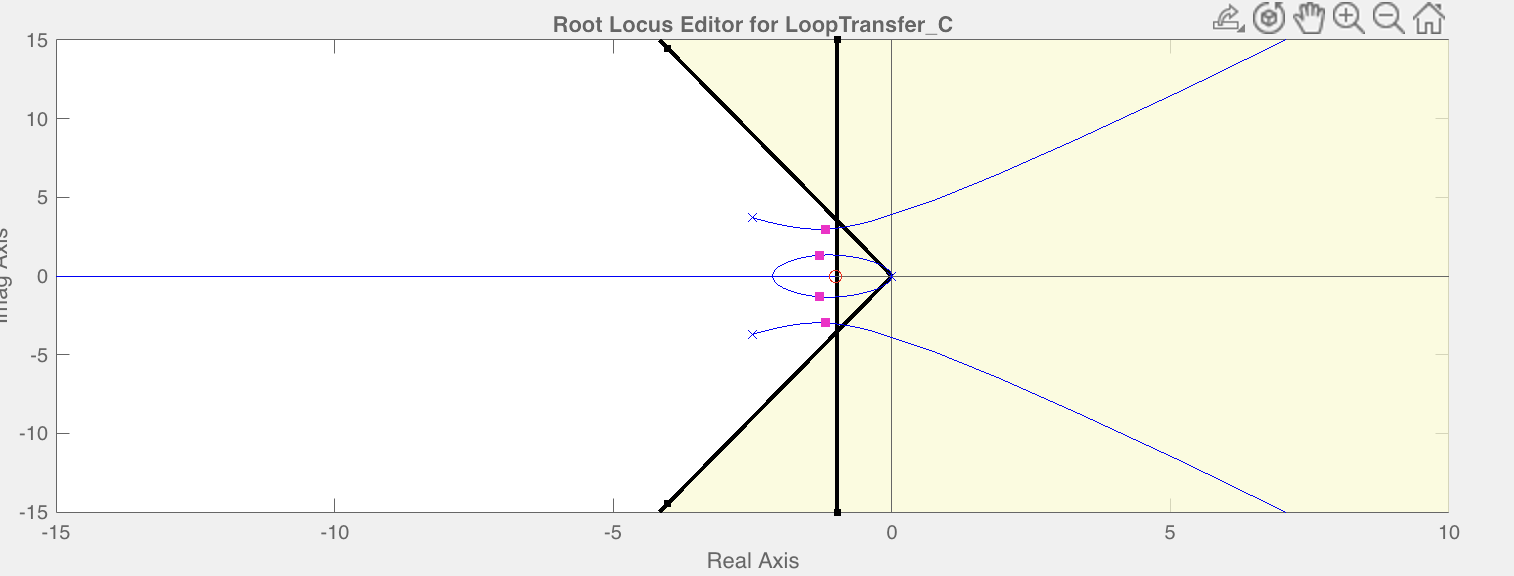
\includegraphics[width=.8\textwidth]{images/dr_2.png}
    \caption{2 Different Constraints}
    \label{fig:dr2}
\end{figure}

As can be seen above, our poles are in the safe zone for all conditions and the step response plot of the system verifies this condition. The step response which illustrates $T_s < 4$ and P.O < 50\% is shown below on Figure \ref{fig:resp}. In this case, $T_s = 3.7 < 4\text{ seconds}$.The $K_p$ and $K_d$ values that correspond to this controller are as follows:
\begin{itemize}
    \item $K_p$ = 355.5
    \item $K_d$ = 375.05
\end{itemize}

\begin{figure}[H]
    \centering
    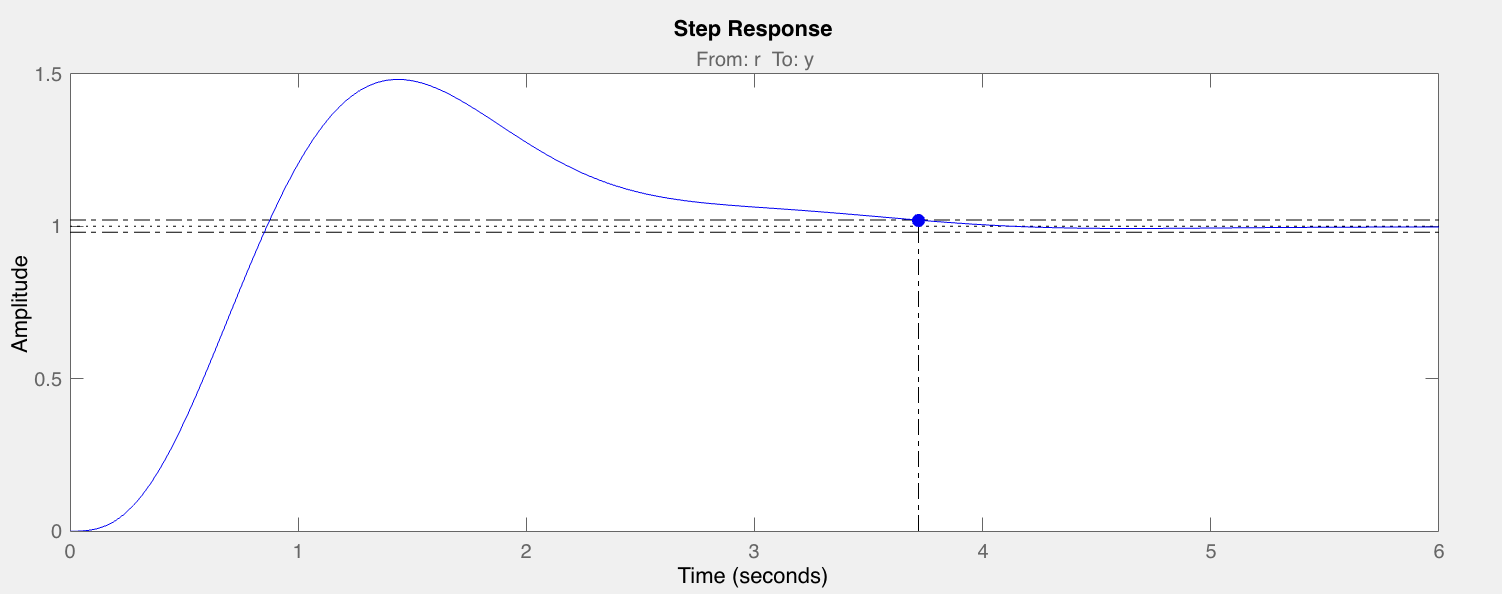
\includegraphics[width=.85\textwidth]{images/ts4.png}
    \caption{Step Response}
    \label{fig:resp}
\end{figure}

\subsection{Building The Simulink Model}

Then, we moved on to Simulink and using block diagrams, we were able to build a model of our system that is connected to the variables on Matlab workspace, using this, we were able continuously update our parameters from Matlab side. Our block diagram model is shown below.

\begin{figure}[H]
    \centering
    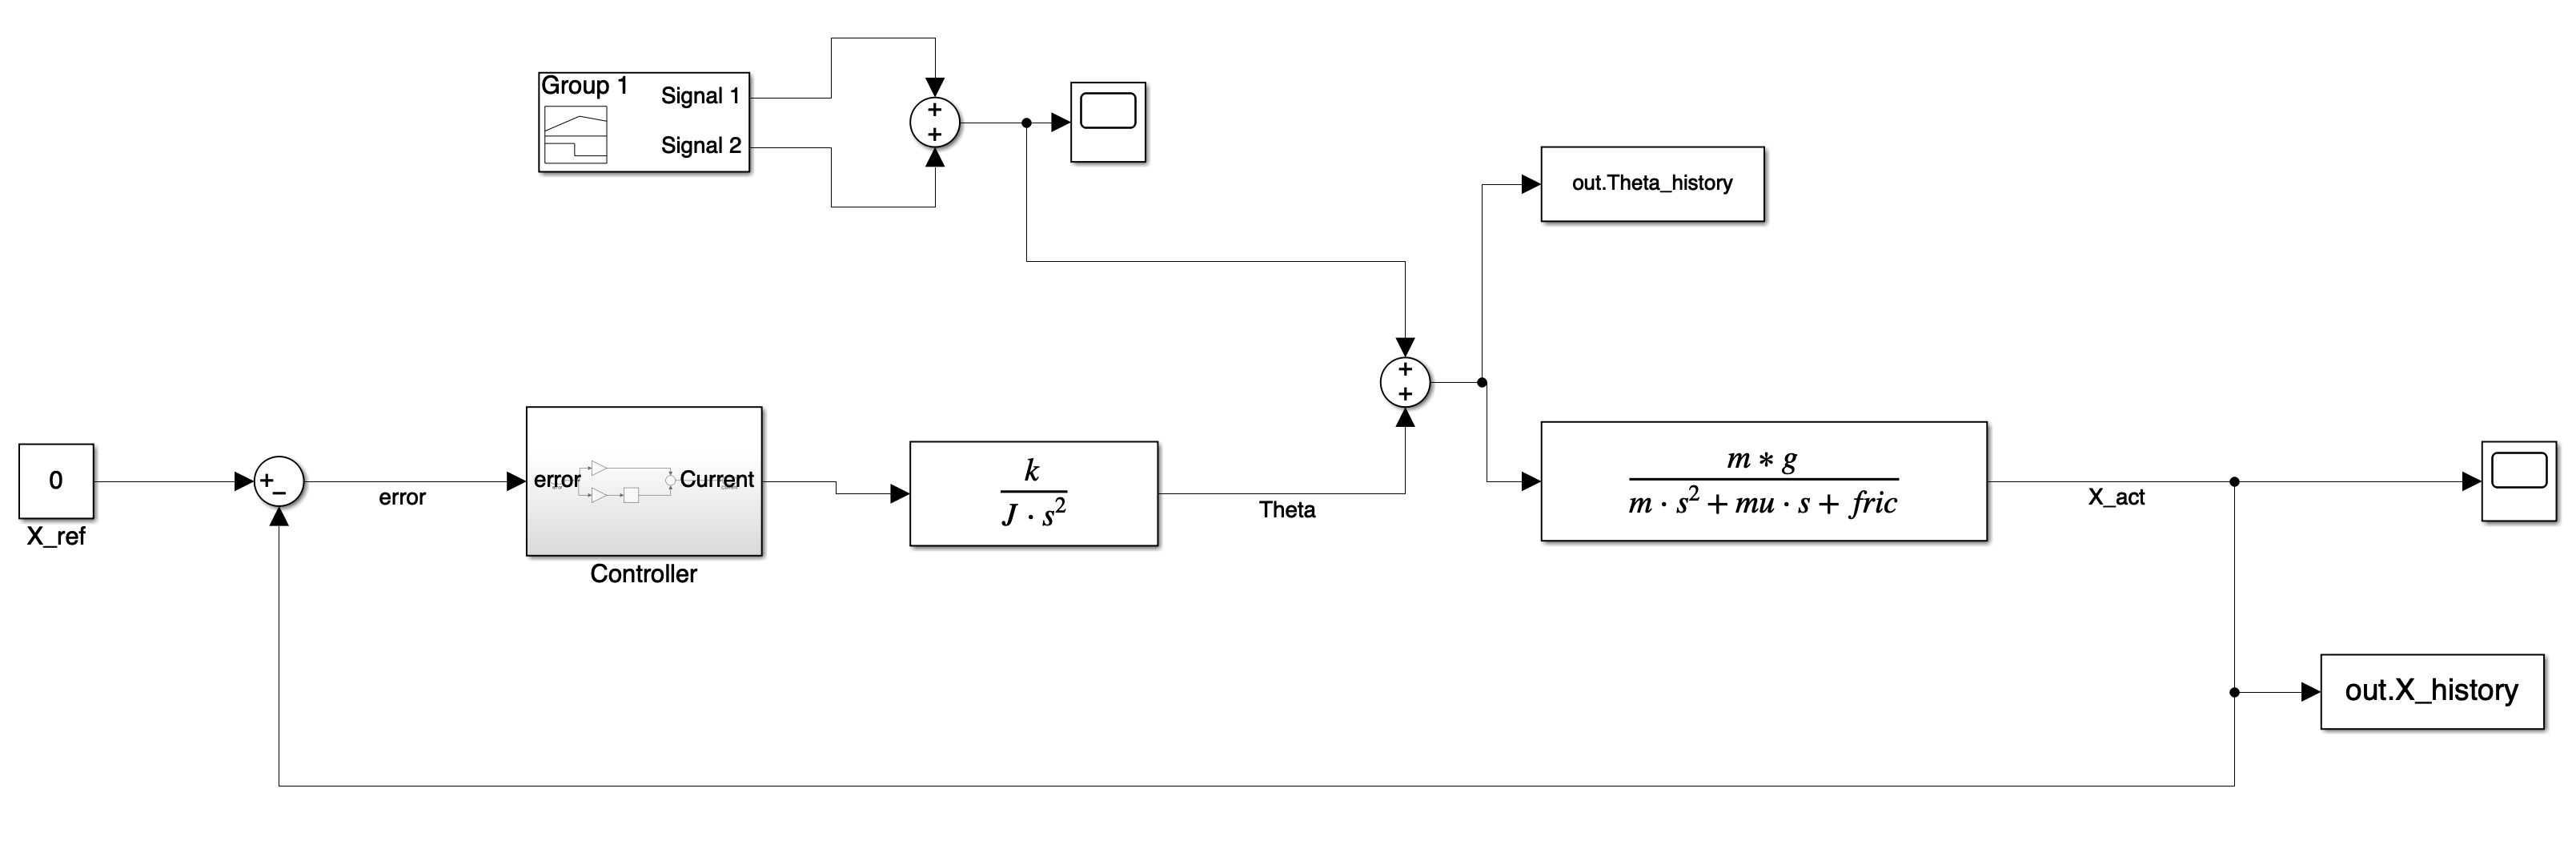
\includegraphics[width=.9\textwidth]{images/sim_model.png}
    \caption{Simulink Model}
    \label{fig:sim_model}
\end{figure}

In this model, our PD controller is created as a subsystem which comprises of the following model shown below. We manually created the controller by summing the $K_p$ and $K_d$ components. While $K_p$ component is more direct, we took the derivative of the signal for $K_d$ the part.

\begin{figure}[H]
    \centering
    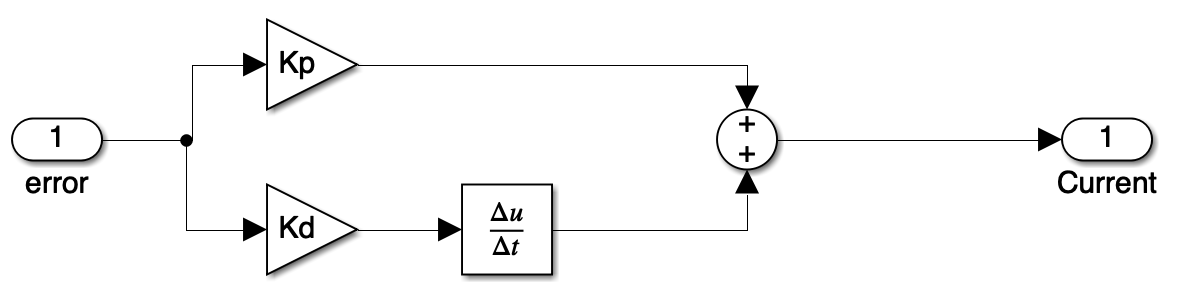
\includegraphics[width=.6\textwidth]{images/pd_ss.png}
    \caption{PD Subsystem}
    \label{fig:pd_ss}
\end{figure}


As Figure \ref{fig:sim_model} illustrates, we have a disturbance signal on our system. This disturbance signal is built using the signal builder and summing that signal with $\Theta$ on Simulink. This allows us to test the performance of our controller better since without it the ball would be stable anyhow. The following figure illustrates our signal. 

\begin{figure}[H]
    \centering
    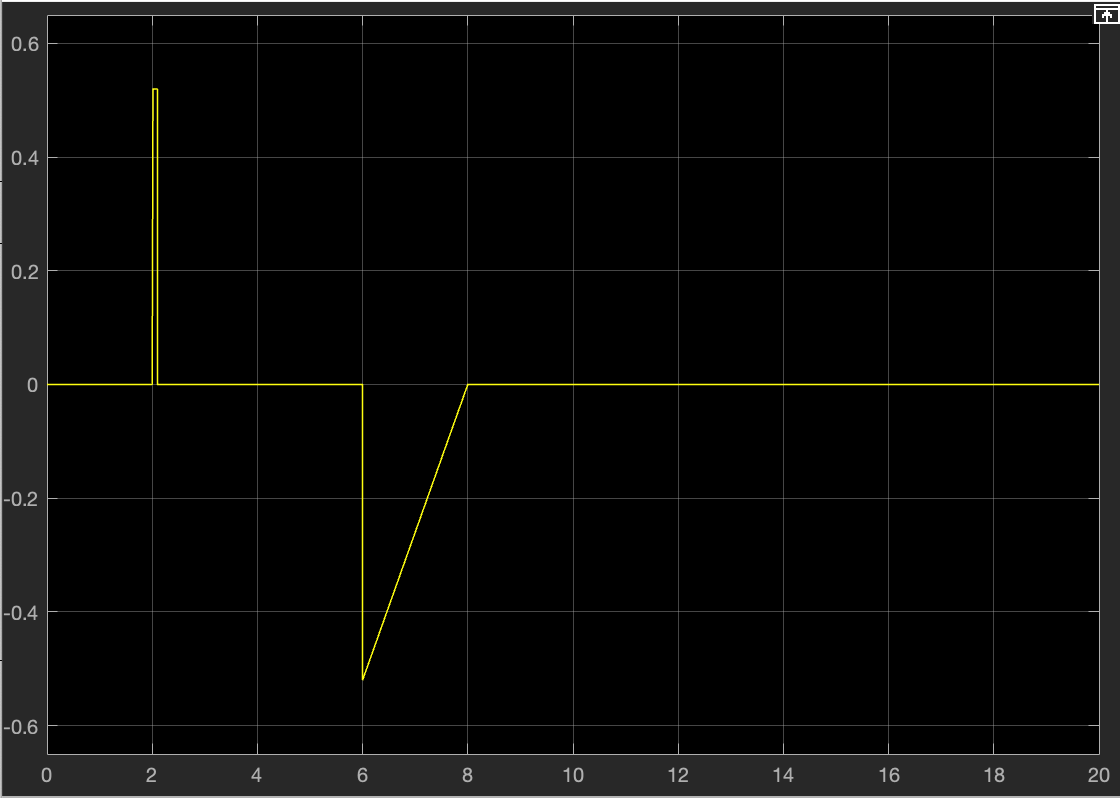
\includegraphics[width=.6\textwidth]{images/dist.png}
    \caption{Disturbance Signal}
    \label{fig:dist}
\end{figure}

Under the discussed disturbance signal, we used scopes to monitor our $\Theta$ and $X$ to check if our system was able to stabilized once the disturbances have been made. Following figures show our $\Theta$ and $X$ respectively.

\begin{figure}[H]
 \centering
\begin{subfigure}{.45\textwidth}
  \centering
  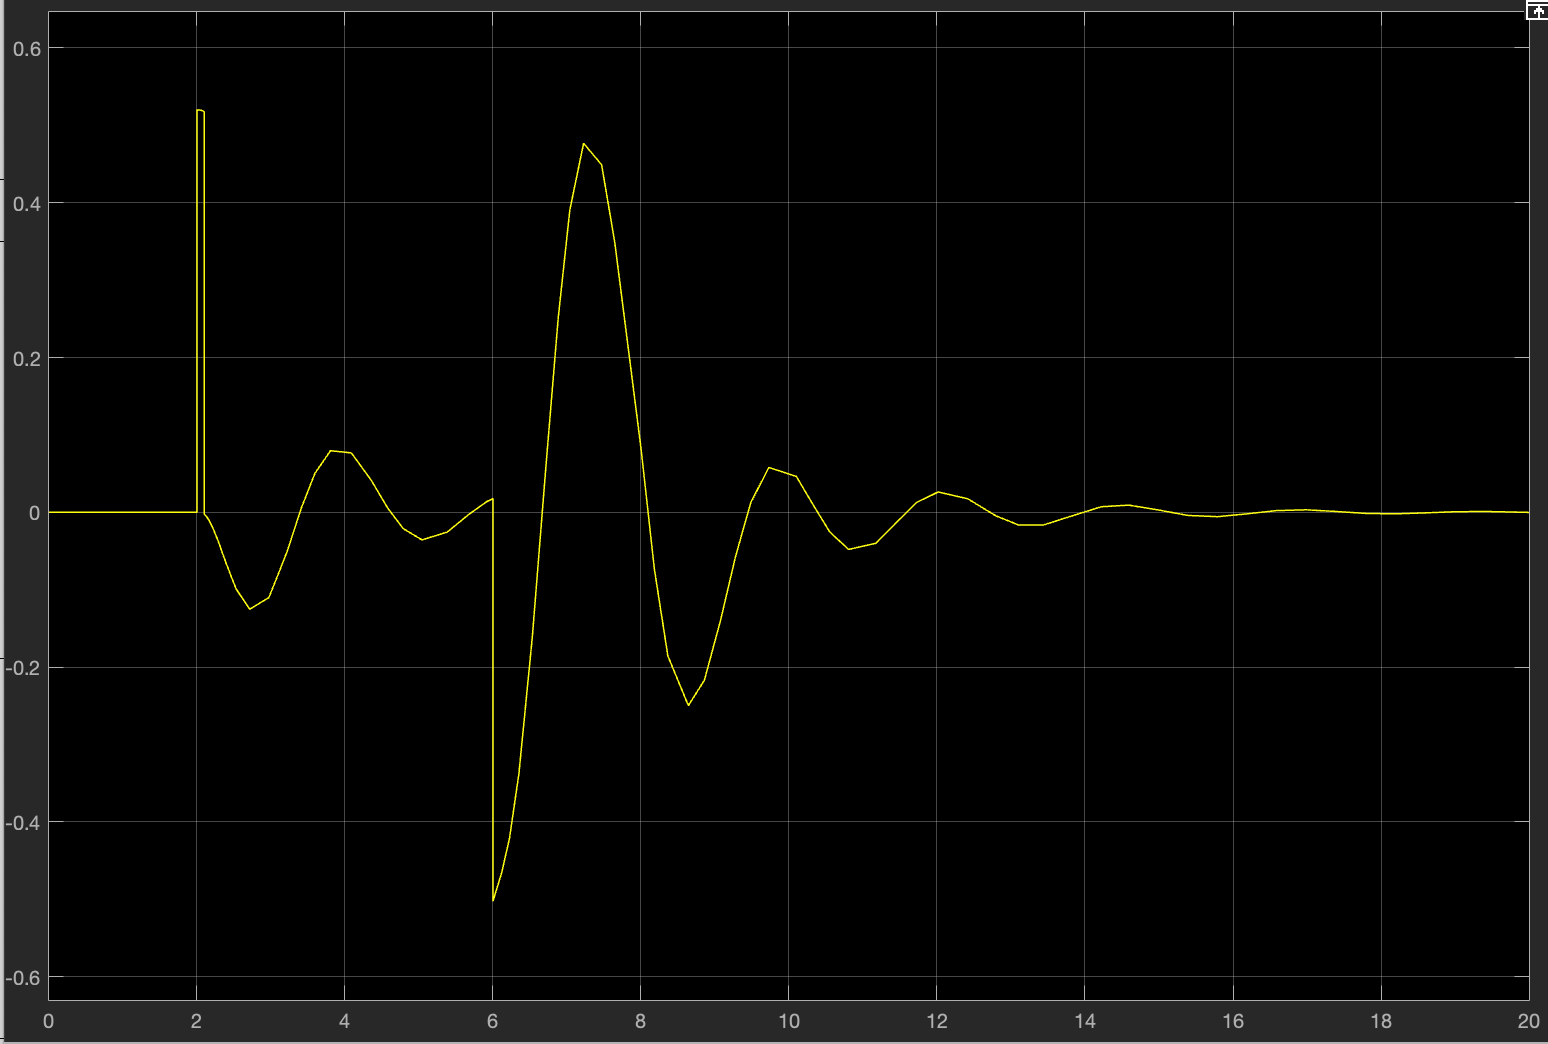
\includegraphics[width=.9\linewidth]{images/regular_theta.png}
  \caption{Scope of $\Theta$}
  \label{fig:x_d_norm}
\end{subfigure}%
~
\begin{subfigure}{.45\textwidth}
  \centering
  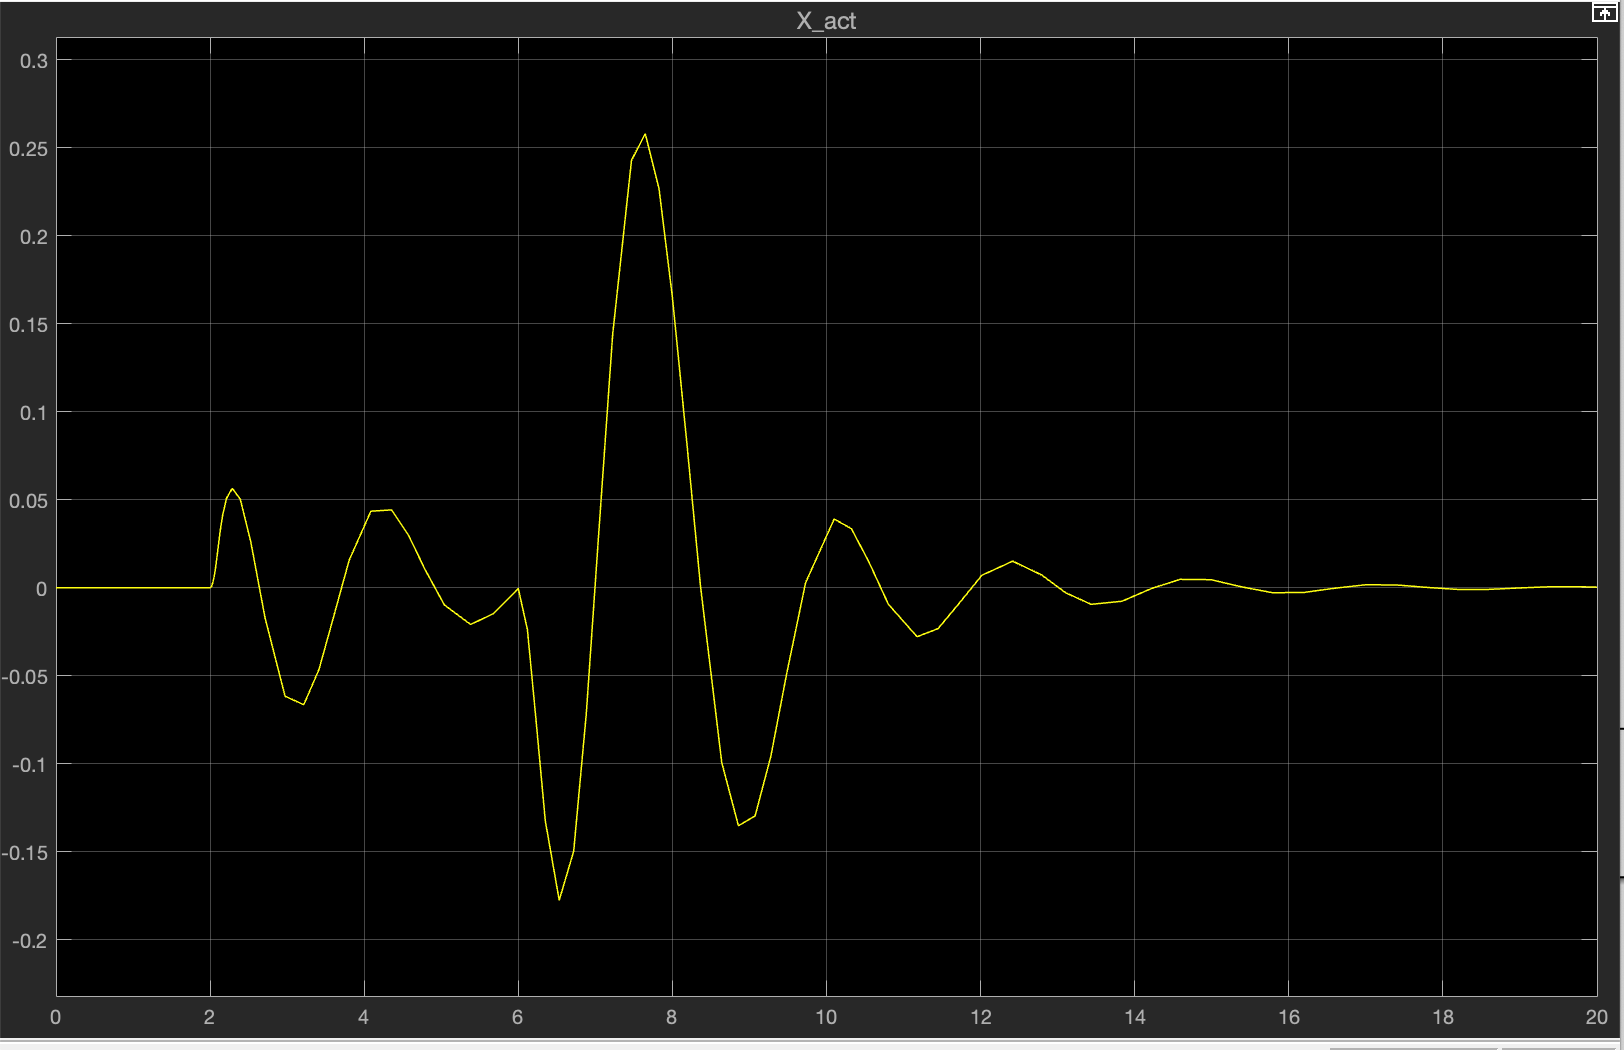
\includegraphics[width=.9\linewidth]{images/regular_x.png}
  \caption{Scope of $X$}
  \label{fig:x_d_norm_actual}
\end{subfigure}
~
\caption{Outputs}
\label{fig:outputs_theta_x}
\end{figure}


Following this, we exported these signals as timeseries datatype and fed into the animation function provided by our TA. With that visualization, we were able to more intuitively observe our system. A sample screenshot from the ending of that animation is shown below.

\begin{figure}[H]
    \centering
    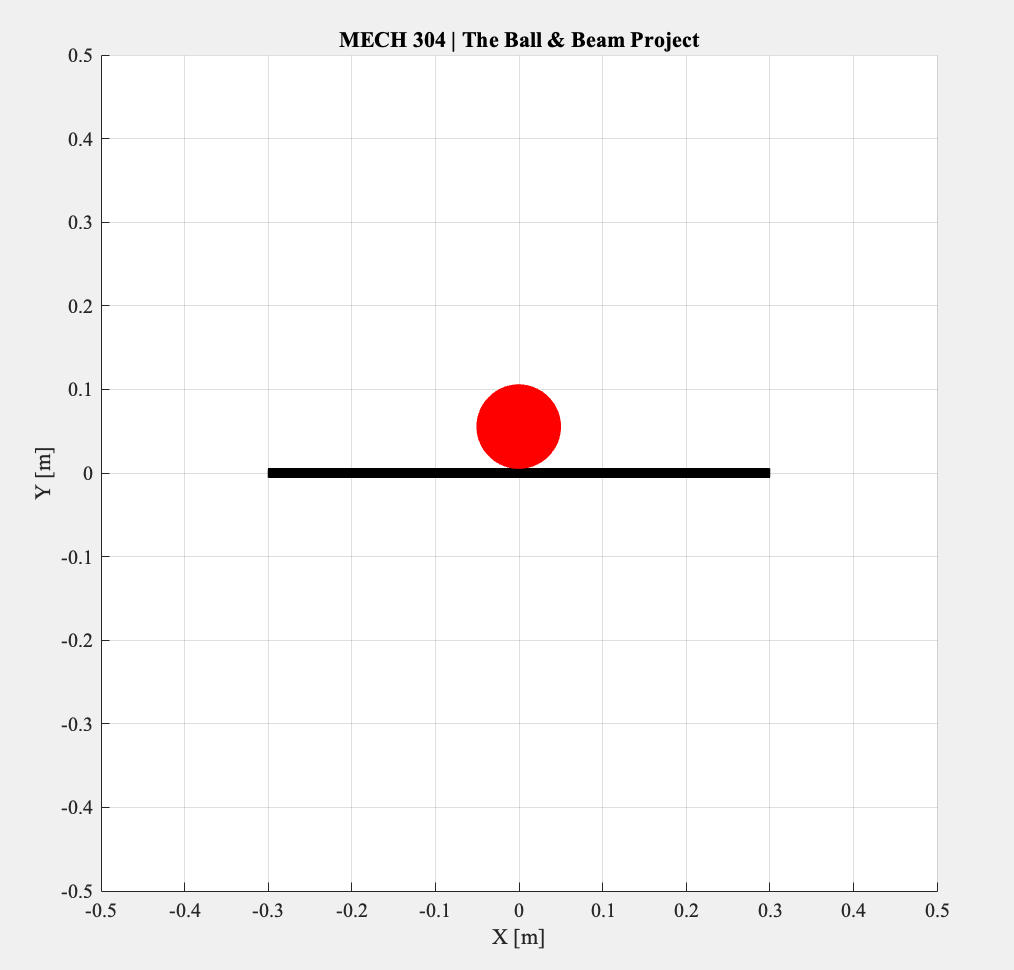
\includegraphics[width=.7\textwidth]{images/anima.png}
    \caption{Stabilized Animation}
    \label{fig:anima}
\end{figure}
